Chiang Mai International School (CMIS) is the oldest school in Chiang Mai and the third oldest international school in Thailand. Missionaries returning to work after World War II established the school for their seven children over sixty years ago. Today CMIS has grown into a diverse international school with over five hundred students originating from over thirty different countries. Despite the expansion, CMIS still promotes the values of Christianity, while warmly welcoming families of all faiths, cultures, and ethnicity. 

For over forty years, CMIS was the only international school in Chiang Mai. Today, international schools are prevalent and CMIS remains a school of choice. With an emphasis on providing academic excellence, in a caring community, CMIS students grow to be confident, articulate learners as well as caring, globally-minded individuals. This commitment has resulted in CMIS being known to many as the best international school in Chiang Mai. This well-deserved reputation is evident in our inspiring students that continue to excel in many areas including the arts, athletics, academics, community service, and leadership. 

The CMIS Focus on Learning Self Study report is the result of several years of collective action, coupled with times of reflection and discussion with teachers, students, staff, parents, and community members. Though the immediate staff and leadership contributed to the construction of the report, CMIS appreciates and honors the work of prior staff and administrative teams. 

CMIS chose the visual parable based on the Indian story entitled Blind Men and the Elephant as the self study mantra. In the story, a group of blind men touch an elephant to learn what it is like. Each one feels a different part, but only one part, such as the side or the tusk. They then compare notes and learn that they are in complete disagreement. The parable reminded CMIS of the importance of considering all viewpoints in obtaining a full picture of reality, and that our perceptions and life experiences can lead to limited access and overreaching misinterpretations. It was a poignant story for CMIS because in the past there had been times when parts of the school were working in isolation of one another. It helped CMIS to continuously focus on creating all the pieces of the report together, no matter how discreet, to best describe the whole. 


\begin{figure}
\centering
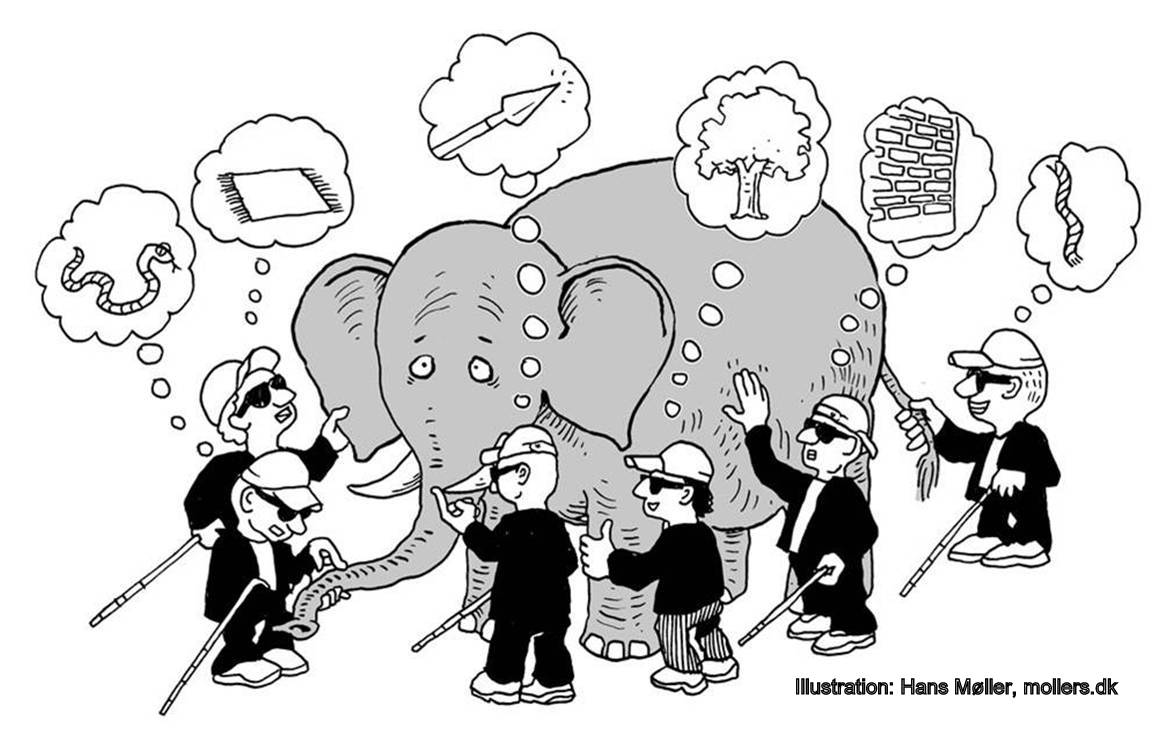
\includegraphics[width=\textwidth]{preface1.jpg}
\caption{Visual Analogy}
\end{figure}

CMIS believes the primary goal of the report is to identify, articulate, and celebrate what CMIS already does to address its most essential institutional goal: increase student learning. This was made clear, early in the self study process, when a staff member suggested that the title of the report was Focus on Learning and that all of our reflections and discussions should be anchored to that idea. From that point forward, CMIS referred to the WASC process and construction of the report as the Focus on Learning. 

An overview and summary given by WASC consultant Barbara Parker officially inaugurated the development of focus and home groups and the collection of self study data in November 2016. This presentation reminded the CMIS team see the report as a valuable self-evaluation tool. Focus on Learning should not be seen as an additional task, only referred to during the accreditation year, but rather as a protocol that guides schools into an ongoing improvement process that includes implementation, assessment, and refinement of the schoolwide planning.

{\centering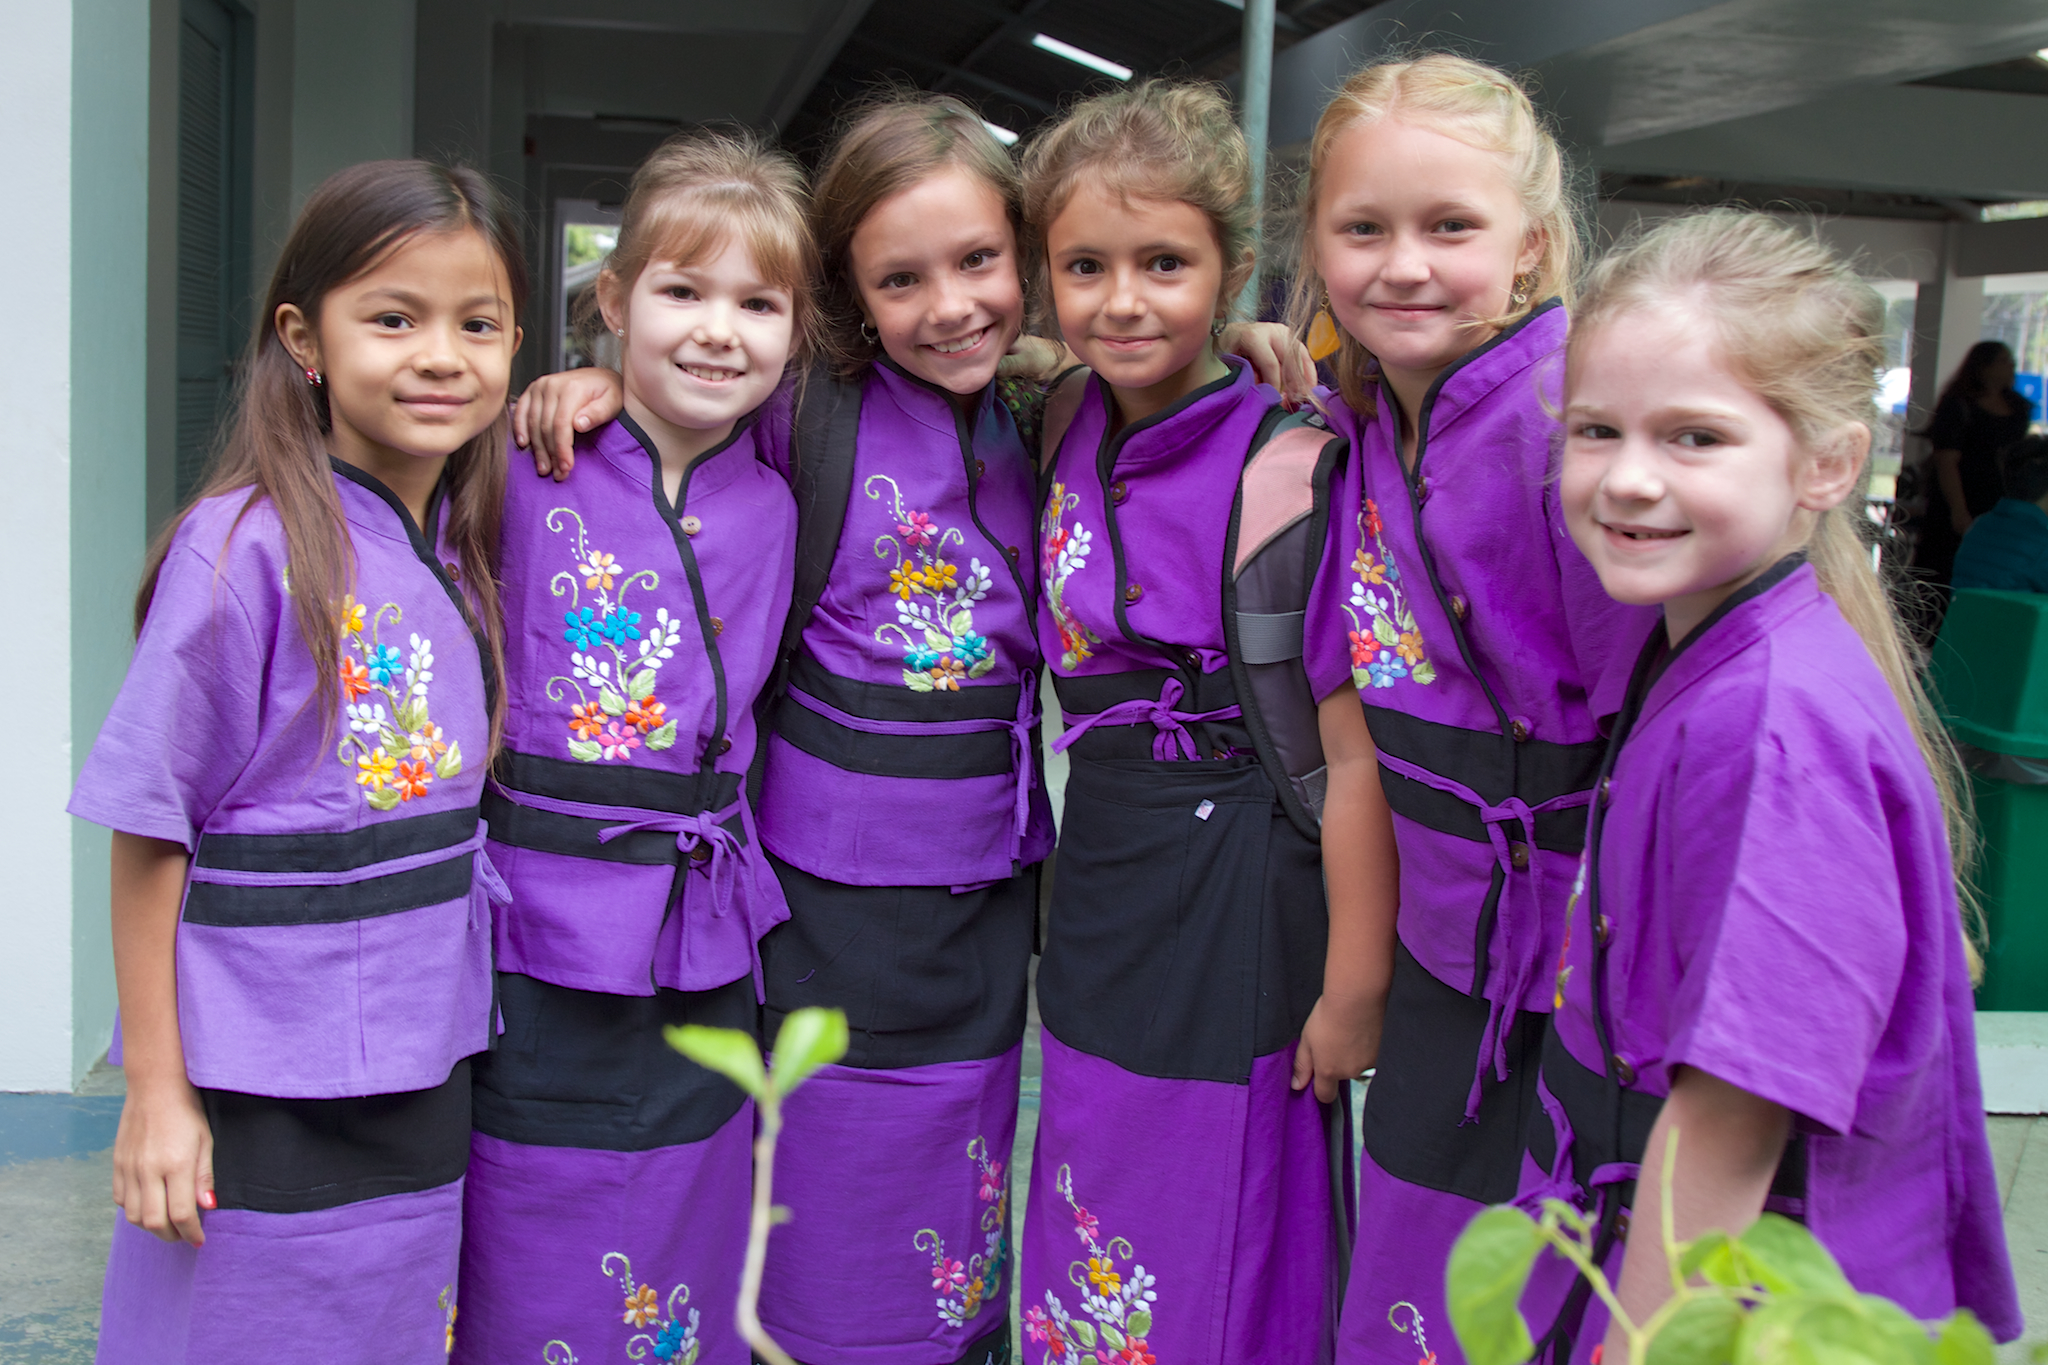
\includegraphics[width=\textwidth]{Preface.jpg}}

Though CMIS has grown significantly since the last self study report in 2011 it has not lost sight of what it does best - “Inspire educational excellence in a caring Christian community that respects and celebrates diversity.” This has been accomplished through a combined effort to redefine the purpose of CMIS goals; improve student achievement and understand that it cannot be achieved without the whole community working together and supporting one another through appreciation, mutual respect, and understanding. This teamwork has brought about the realignment of standards, curriculum, and instructional practices that are research based and anchored in 21st century skills. It has enabled the school divisions to participate in vertical and horizontal articulation that has resulted in stronger coherence. It has encouraged leadership to be a shared responsibility, where students, parents and staff have a collective voice and authentic opportunities to reflect on school practices, create meaningful plans for improvement, and seek effective ways to track progress. Most importantly, it has created a sense of cohesiveness and an understanding that self improvement is a healthy process that is ongoing and essential in order to meet the diverse needs of CMIS students.



